\chapter{Pulse Wave Solver}

\section{Synopsis}

1D modelling of the vasculature (arterial network) represents and insightful and efficient tool for tackling problems encountered in arterial biomechanics as well as other engineering problems. In particular, 3D modelling of the vasculature is relatively expensive. 1D modelling provides an alternative in which the modelling assumptions provide a good balance between physiological accuracy and computational efficiency. To describe the flow and pressure in this network we consider the conservation of mass and momentum applied to an impermeable, deformable tube filled with an incompressible fluid, the nonlinear system of partial differential equations presented in non-conservative form is given by

\begin{equation}
\label{eqn:1DContMom}
\frac{\partial \mathbf{U}}{\partial{t}} + \mathbf{H}\frac{\partial{\mathbf{U}}}{\partial{x}}
= \mathbf{S}
\end{equation}

\begin{equation}
\mathbf{U}=\begin{bmatrix} U \\ A \end{bmatrix}, \quad \mathbf{H}=\begin{bmatrix} U & A \\ \rho\frac{\partial{P}}{\partial{A}} & U\end{bmatrix}, \quad \mathbf{S}=\begin{bmatrix} 0 \\ \frac{1}{\rho}\left(\frac{f}{A}-s\right) \end{bmatrix} \nonumber
\end{equation}

in which $A$ is the Area (related to pressure), $x$ is the axial coordinate along the vessel, $U(x,t)$ the axial velocity, $P(x,t)$ is the pressure in the tube,  $\rho$ is the density and finally $f$ the frictional force per unit length. The unknowns in Eq. \ref{eqn:1DContMom} are $U, A$ and $P$; hence, we must provide an explicit algebraic relationship to close this system. Typically, closure is provided by an algebraic relationship between $A$ and $P$. For a thin, viscoelastic tube this is given by

\begin{equation}
P=P_{0}+\beta\left(\sqrt{A}-\sqrt{A_{0}}\right) + \frac{\Gamma}{\sqrt{A}}\frac{\partial A}{\partial t}, \quad \beta=\frac{\sqrt{\pi}E h }{(1-\nu^{2})A_{0}}, \quad \Gamma = \frac{2\sqrt{\pi} \varphi h}{3A_{0}}
\label{eqn:PA}
\end{equation}

where $P_{0}$ is the external pressure, $A_{0}$ is the initial cross-sectional area, $E$ is the Young's modulus, $h$ is the vessel wall thickness, $\nu$ is the Poisson's ratio, and $\varphi$ is the wall viscosity. An empirical law has also been implemented that incorporates strain-stiffening through the parameter $\alpha$ [1]:

\begin{equation}
	\label{eqn:EmpiricalLaw}
    P = P_{0} - \frac{\beta \sqrt{A_{0}}}{2\alpha}\ln{\left[1 - \alpha\ln{\left(\frac{A}{A_{0}}\right)}\right]} + \frac{\Gamma}{\sqrt{A}}\frac{\partial A}{\partial t}.
\end{equation}

Application of Riemann's method of characteristics to Eqs. \eqref{eqn:1DContMom} and \eqref{eqn:PA} indicates that velocity and area are propagated through the system by forward and backward travelling waves. These waves are reflected and within the network by appropriate treatment of interfaces and boundaries. In the following, we will explain the usage of the blood flow solver on the basis of a single-artery problem and
also on an arterial network consisting of $55$ arteries.

\section{Usage}
\begin{lstlisting}[style=BashInputStyle]
PulseWaveSolver session.xml
\end{lstlisting}

\section{Session file configuration}

\subsection{Pulse Wave Solver mesh connectivity}
Typically 1D arterial networks are made up of a connection of different base units: segments, bifurcations and merging junctions. The input format in the PulseWaveSolver means these connections are handle naturally from the mesh topology; hence care must be taken when designing the 1D domain. The figure below outlines the structure of a bifurcation, which is a common reoccurring structure in the vasculature.

\begin{figure}
\begin{center}
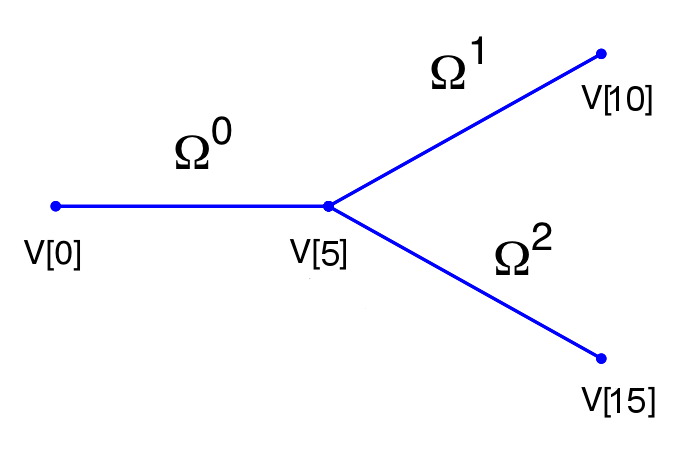
\includegraphics[width=7cm]{img/PulseWaveBifurcation.png}
\caption{Model of bifurcating artery. The bifurcation is made of three domains and 15 vertices. Vertex V[0] is the inlet and vertices V[10] and V[15] the outlets.}
\end{center}
\end{figure}

To represent this topology in the xml file we specify the following vertices under the section \inltt{VERTEX} (the extents are: $-100 \geq x \leq 100$ and $-100 \geq y \leq 100$ )

\begin{lstlisting}[style=XmlStyle]
<VERTEX>
  <V ID="0">-1.000e+02 0.000e+00 0.000e+00</V>
  <V ID="1">-8.000e+01 0.000e+00 0.000e+00</V>
  <V ID="2">-6.000e+01 0.000e+00 0.000e+00</V>
  <V ID="3">-4.000e+01 0.000e+00 0.000e+00</V>
  <V ID="4">-2.000e+01 0.000e+00 0.000e+00</V>
  <V ID="5"> 0.000e+00 0.000e+00 0.000e+00</V>

  <V ID="6"> 2.000e+01 2.000e+01 0.000e+00</V>
  <V ID="7"> 4.000e+01 4.000e+01 0.000e+00</V>
  <V ID="8"> 6.000e+01 6.000e+01 0.000e+00</V>
  <V ID="9"> 8.000e+01 8.000e+01 0.000e+00</V>
  <V ID="10"> 1.000e+02 1.000e+02 0.000e+00</V>

  <V ID="11"> 2.000e+01 -2.000e+01 0.000e+00</V>
  <V ID="12"> 4.000e+01 -4.000e+01 0.000e+00</V>
  <V ID="13"> 6.000e+01 -6.000e+01 0.000e+00</V>
  <V ID="14"> 8.000e+01 -8.000e+01 0.000e+00</V>
  <V ID="15"> 1.000e+02 -1.000e+02 0.000e+00</V>
</VERTEX>
\end{lstlisting}

The elements from these vertices are then constructed under the section \inltt{ELEMENT} by defining
\begin{lstlisting}[style=XmlStyle]
<ELEMENT>
  <!-- Parent artery -->
  <S ID="0">    0     1 </S>
  <S ID="1">    1     2 </S>
  <S ID="2">    2     3 </S>
  <S ID="3">    3     4 </S>
  <S ID="4">    4     5 </S>
  <!-- Daughter artery 1 -->
  <S ID="5">    5     6 </S>
  <S ID="6">    6     7 </S>
  <S ID="7">    7     8 </S>
  <S ID="8">    8     9 </S>
  <S ID="9">    9     10 </S>
  <!-- Daughter artery 2 -->
  <S ID="11">     5     11 </S>
  <S ID="12">    11    12 </S>
  <S ID="13">    12    13 </S>
  <S ID="14">    13    14 </S>
  <S ID="15">    14    15 </S>
</ELEMENT>
\end{lstlisting}

The composites, which represent groups of elements and boundary regions are defined under the section \inltt{COMPOSITE} by
\begin{lstlisting}[style=XmlStyle]
<COMPOSITE>
  <C ID="0"> S[0-4] </C>	<!-- Parent artery -->
  <C ID="1"> V[0] </C>		<!-- Inlet to domain -->

  <C ID="3"> S[5-9] </C>	<!-- Daughter artery 1 -->
  <C ID="4"> V[10] </C>		<!-- Outlet of daughter artery 1 -->

  <C ID="6"> S[11-15] </C>	<!-- Daughter artery 2 -->
  <C ID="8"> V[15] </C>		<!-- Outlet of daughter artery 2 -->
</COMPOSITE>
\end{lstlisting}

Each of the segments can be then represented under the section \inltt{DOMAIN} by
\begin{lstlisting}[style=XmlStyle]
<DOMAIN>
  <D ID="0"> C[0] </D>	<!-- Parent artery -->
  <D ID="1"> C[3] </D>	<!-- Daughter artery 1 -->
  <D ID="2"> C[6] </D>	<!-- Daughter artery 2 -->
</DOMAIN>
\end{lstlisting}

We will use the different domains later to define variable material properties and cross-sectional areas.

\subsection{Time Integration Scheme}

\begin{itemize}
\item \inltt{Method} the time-stepping method.
\item \inltt{Variant} the variant to the method. 
\item \inltt{Order} the order of the method.
\item \inltt{FreeParameters} any free parameters required.
\end{itemize}

\subsection{Session Info}
The PulseWaveSolver is specified through the \inltt{EquationType}
option in the session file. This can be set as follows:
\begin{itemize}
\item \inltt{Projection}: Only a discontinuous projection can be specified
using the following option:
    \begin{itemize}
    \item \inltt{Discontinuous} for a discontinous Galerkin (DG) projection.
    \end{itemize}
\item \inltt{UpwindTypePulse}:
    \begin{itemize}
    \item \inltt{UpwindPulse}
    \end{itemize}
\item \inltt{OutputExtraFields}:
    \begin{itemize}
    \item \inltt{True} returns the wave speed and both characteristics
    \end{itemize}
\item \inltt{PressureArea}:
    \begin{itemize}
    \item \inltt{Beta} for Eq. \eqref{eqn:PA}
    \item \inltt{Empirical} for Eq. \eqref{eqn:EmpiricalLaw}
    \end{itemize}
\end{itemize}

 \subsection{Parameters}
The following parameters can be specified in the \inltt{PARAMETERS} section of
the session file.
\begin{itemize}
\item \inltt{TimeStep} is the time-step size;
\item \inltt{FinTime} is the final physical time at which the simulation will  stop;
\item \inltt{NumSteps} is the equivalent of \inltt{FinTime} but instead of specifying the
physical final time the number of time-steps is defined;
\item \inltt{IO\_CheckSteps} sets the number of steps between successive checkpoint files;
\item \inltt{IO\_InfoSteps} sets the number of steps between successive info stats are printed
to screen;
\item \inltt{rho} density of the fluid. Default value = 1.0;
\item \inltt{nue} Poisson's ratio. Default value = 0.5 ;
\item \inltt{pext} external pressure. Default value = 0;
\item \inltt{pout} outflow pressure to the venous system for the terminal boundary conditions. Default value = 0;
\item \inltt{h0} wall thickness. Default value = 1.0;
\end{itemize}

\subsection{Boundary conditions}
In this section we can specify the boundary conditions for our problem.
First we need to define the variables under the section \inltt{VARIABLES}.
\begin{lstlisting}[style=XmlStyle]
<VARIABLES>
   <V ID="0"> A </V>
   <V ID="1"> u </V>
</VARIABLES>
\end{lstlisting}

The composites that we want to apply out boundary conditions then need to be defined in the \inltt{BOUNDARYREGIONS}, for example if we had three composites (C[1], C[4] and C[8]) that correspond to three vertices of the computational mesh we would define:
\begin{lstlisting}[style=XmlStyle]
<BOUNDARYREGIONS>
  <B ID="0"> C[1] </B>
  <B ID="1"> C[4] </B>
  <B ID="2"> C[8] </B>
 </BOUNDARYREGIONS>
\end{lstlisting}

Finally we can specify the boundary conditions on the regions specified under \inltt{BOUNDARYREGIONS}.

The Pulse Wave Solver comes with a number of boundary conditions that are unique to this solver. Boundary conditions must be provided for both the area and velocity at the inlets and outlets of the domain. Examples of the different boundary conditions will be provided in the following.

\paragraph{Inlet boundary condition:~} The inlet condition may be specified algebraically in four different ways: as an area variation (\inltt{A-inflow}); a velocity profile (\inltt{U-inflow}); a volume flux (\inltt{Q-inflow}); or by prescribing the forward characteristic (\inltt{TimeDependent}). When prescribing a volume flux, it must be specified in the input file via the area, as illustrated below. Note that $u = 1.0$.

\begin{lstlisting}[style=XmlStyle]
<REGION REF="0">
	<D VAR="A" USERDEFINEDTYPE="Q-inflow" VALUE="(7.112e-4)*(sin(7.854*t)
-0.562)*(1/(1+exp(-400*(sin(7.854*t)-0.562))))" />
        <D VAR="u" USERDEFINEDTYPE="Q-inflow" VALUE="1.0" />
</REGION>
\end{lstlisting}

\paragraph{Terminal boundary conditions:~} At the outlets of the domain there are four possible boundary conditions: reflection (\inltt{Terminal}), terminal resistance \inltt{R-terminal},
Two element windkessel (CR)  \inltt{CR-terminal}, and three element windkessel (RCR) \inltt{RCR-terminal}.  An example of the outflow boundary condition of the RCR terminal is given below
\begin{lstlisting}[style=XmlStyle]
<REGION REF="1">
	<D VAR="A" USERDEFINEDTYPE="RCR-terminal" VALUE="RT" />
	<D VAR="u" USERDEFINEDTYPE="RCR-terminal" VALUE="C" />
</REGION>
\end{lstlisting}
Where \inltt{RT} is the total peripheral resistance  used in the the  \inltt{R-terminal}, \inltt{CR-terminal} and \inltt{RCR-terminal}  models

\subsection{Functions}

The following functions can be specified inside the \inltt{CONDITIONS} section
of the session file:
\begin{itemize}
\item \inltt{MaterialProperties}: specifies $\beta$ for each domain.
\item \inltt{A\textunderscore0}: specifies $A_{0}$ for each domain as used in the tube law.
\item \inltt{Viscoelasticity}: specifies $\Gamma$ for each domain. Defaults to zero for every artery if not included.
\item \inltt{StrainStiffening}: specifies $\alpha$ for each domain for Eq. \eqref{eqn:EmpiricalLaw}. Defaults to 0.5 for every artery if not included.
\item \inltt{AdvectionVelocity}: specifies the advection velocity $v$.
\item \inltt{InitialConditions}: specifies the initial condition for unsteady
 problems.
\item \inltt{Forcing}: specifies the forcing function $f$
\end{itemize}

As an example to specify the material properties for each domain in the previous bifurcation example we would enter:
\begin{lstlisting}[style=XmlStyle]
<FUNCTION NAME="MaterialProperties">
   <E VAR="beta" DOMAIN="0" VALUE="97" />
   <E VAR="beta" DOMAIN="1" VALUE="87" />
   <E VAR="beta" DOMAIN="2" VALUE="233" />
</FUNCTION>
\end{lstlisting}

The values of \inltt{beta} are used in the pressure-area relationship (Eq. \eqref{eqn:PA}).

\section{Examples}

\subsection{Human Vascular Network}
The PulseWaveSolver is also capable of handling more complex networks, such as
a complete human arterial tree proposed by Westerhof et al. \cite{We69}.
In this example, we will use the refined data from \cite{ShFoPeFr03} and set up
the network shown in the figure in the right. We will explain how bifurcations
are set correctly and how each arterial segment gets its correct physiological
data.

\begin{figure}
	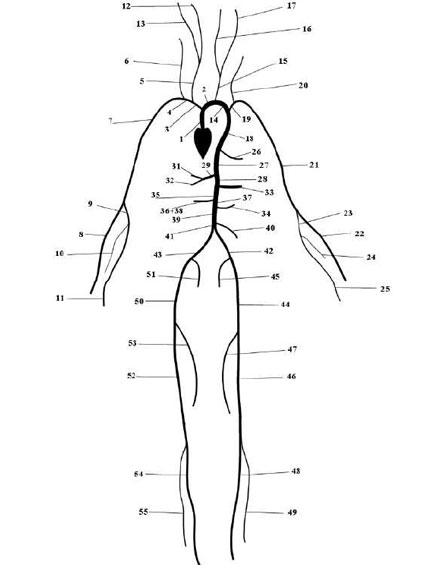
\includegraphics[width=0.49\linewidth]{img/55_artery_network.jpg}
	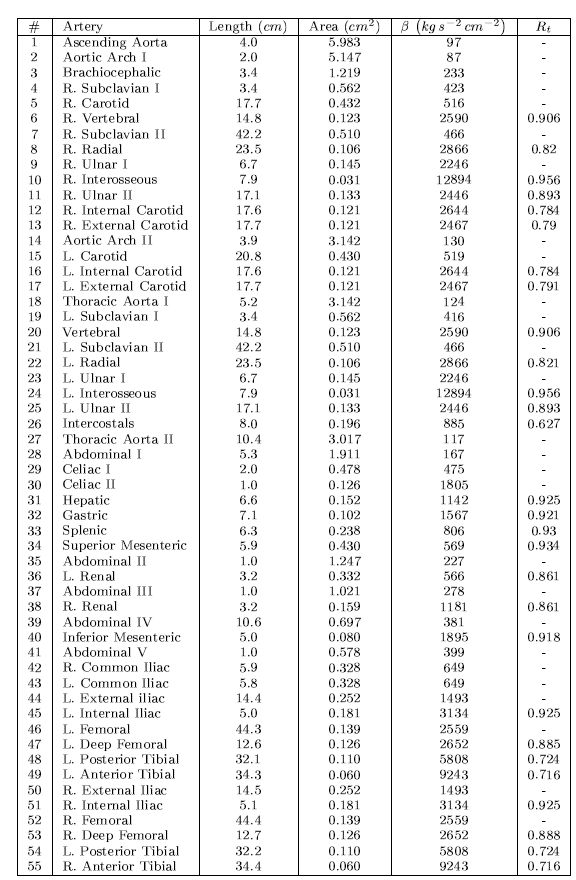
\includegraphics[width=0.49\linewidth]{img/Data_Table.png}
\end{figure}

First, we will set up the mesh where each arterial segment is represented by one
element and two vertices respectively. Then, we will subdivide the mesh into
different subdomains by using the \inltt{<COMPOSITE>} section. Here, each
arterial segment is described by the contained elements and its first and last
vertex.

The mesh connectivity is specified during the creation of elements by indicating
the starting vertex and ending vertex of each individual artery segment. Shared
vertices are used to describe bifurcations, junctions and mergers between
different artery segments in the network.

The composites are then used to specify the two adjoining segments of an artery,
where the first segment merely allows for description of the connectivity.

\begin{lstlisting}[style=XmlStyle]
<GEOMETRY DIM="1" SPACE="1">
    <VERTEX>
        <V ID="0"> 0.000e+00 0.000e+00 0.000e+00</V> <!-- 1 -->
        <V ID="1"> 4.000e+00 0.000e+00 0.000e+00</V>

        <V ID="2"> 4.000e+00 0.000e+00 0.000e+00</V> <!-- 2 -->
        <V ID="3"> 6.000e+00 0.000e+00 0.000e+00</V>

        <V ID="4"> 4.000e+00 0.000e+00 0.000e+00</V> <!-- 3 -->
        <V ID="5"> 7.400e+00 0.000e+00 0.000e+00</V>
           .
           .
           .
        <V ID="108"> 109.100e+00 -45.000e+00 0.000e+00</V> <!-- 55 -->
        <V ID="109"> 143.500e+00 -45.000e+00 0.000e+00</V>
    </VERTEX>
    <ELEMENT>
        <S ID="0">    0     1 </S>
        <S ID="1">    1     2 </S>
        <S ID="2">    1     4 </S>
        <S ID="3">    2     3 </S>
        <S ID="4">    4     5 </S>
        <S ID="5">    5     6 </S>
        <S ID="6">    5     8 </S>
        <S ID="7">    6     7 </S>
        <S ID="8">    8     9 </S>
          .
          .
          .
        <S ID="106">   103    108 </S>
        <S ID="107">   108    109 </S>
        <S ID="108">   85    98 </S>
    <ELEMENT>
    <COMPOSITE>
        <C ID="0"> S[0] </C> <!-- 1 -->
        <C ID="1"> V[0] </C>
        <C ID="2"> V[1] </C>

        <C ID="3"> S[1,3] </C> <!-- 2 -->
        <C ID="4"> V[2] </C>
        <C ID="5"> V[3] </C>

        <C ID="6"> S[2,4] </C> <!-- 3 -->
        <C ID="7"> V[4] </C>
        <C ID="8"> V[5] </C>
           .
           .
           .
        <C ID="162"> S[106,107] </C> <!-- 55 -->
        <C ID="163"> V[108] </C>
        <C ID="164"> V[109] </C>
    </COMPOSITE>
</GEOMETRY>
\end{lstlisting}

Then the choice of polynomial order, solver information, area of the arteries
and other parameters are specified.

\begin{lstlisting}[style=XmlStyle]
<EXPANSIONS>
    <E COMPOSITE="C[0]" NUMMODES="5" FIELDS="A,u" TYPE="MODIFIED" />
    <E COMPOSITE="C[3]" NUMMODES="5" FIELDS="A,u" TYPE="MODIFIED" />
       ...

    <E COMPOSITE="C[162]" NUMMODES="5" FIELDS="A,u" TYPE="MODIFIED" />
</EXPANSIONS>

<CONDITIONS>

    <PARAMETERS>

        <P> TimeStep       = 1e-4               </P>
        <P> FinTime        = 1.0              </P>
        <P> NumSteps       = FinTime/TimeStep   </P>
        <P> IO_CheckSteps  = NumSteps/50        </P>
           ...
        <P> A53            = 0.126              </P>
        <P> A54            = 0.110              </P>
        <P> A55            = 0.060              </P>
    </PARAMETERS>

    <TIMEINTEGRATIONSCHEME>
        <METHOD> RungeKutta </METHOD>
        <VARIANT> SSP </VARIANT>
        <ORDER> 2 </ORDER>
    </TIMEINTEGRATIONSCHEME>
        
    <SOLVERINFO>
        <I PROPERTY="EQTYPE" VALUE="PulseWavePropagation" />
        <I PROPERTY="Projection" VALUE="DisContinuous" />
        <I PROPERTY="TimeIntegrationMethod" VALUE="RungeKutta2_ImprovedEuler" />
        <I PROPERTY="UpwindTypePulse"  VALUE="UpwindPulse"/>
    </SOLVERINFO>

    <VARIABLES>
        <V ID="0"> A </V>
        <V ID="1"> u </V>
    </VARIABLES>

\end{lstlisting}

The vertices where the network terminates are specified as boundary regions
based on their subsequent composite ids.

\begin{figure}
	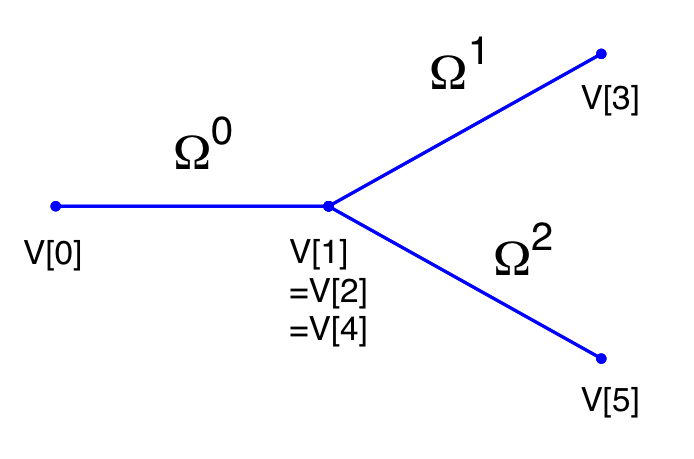
\includegraphics[width=0.49\linewidth]{img/Bifurcation.png}
	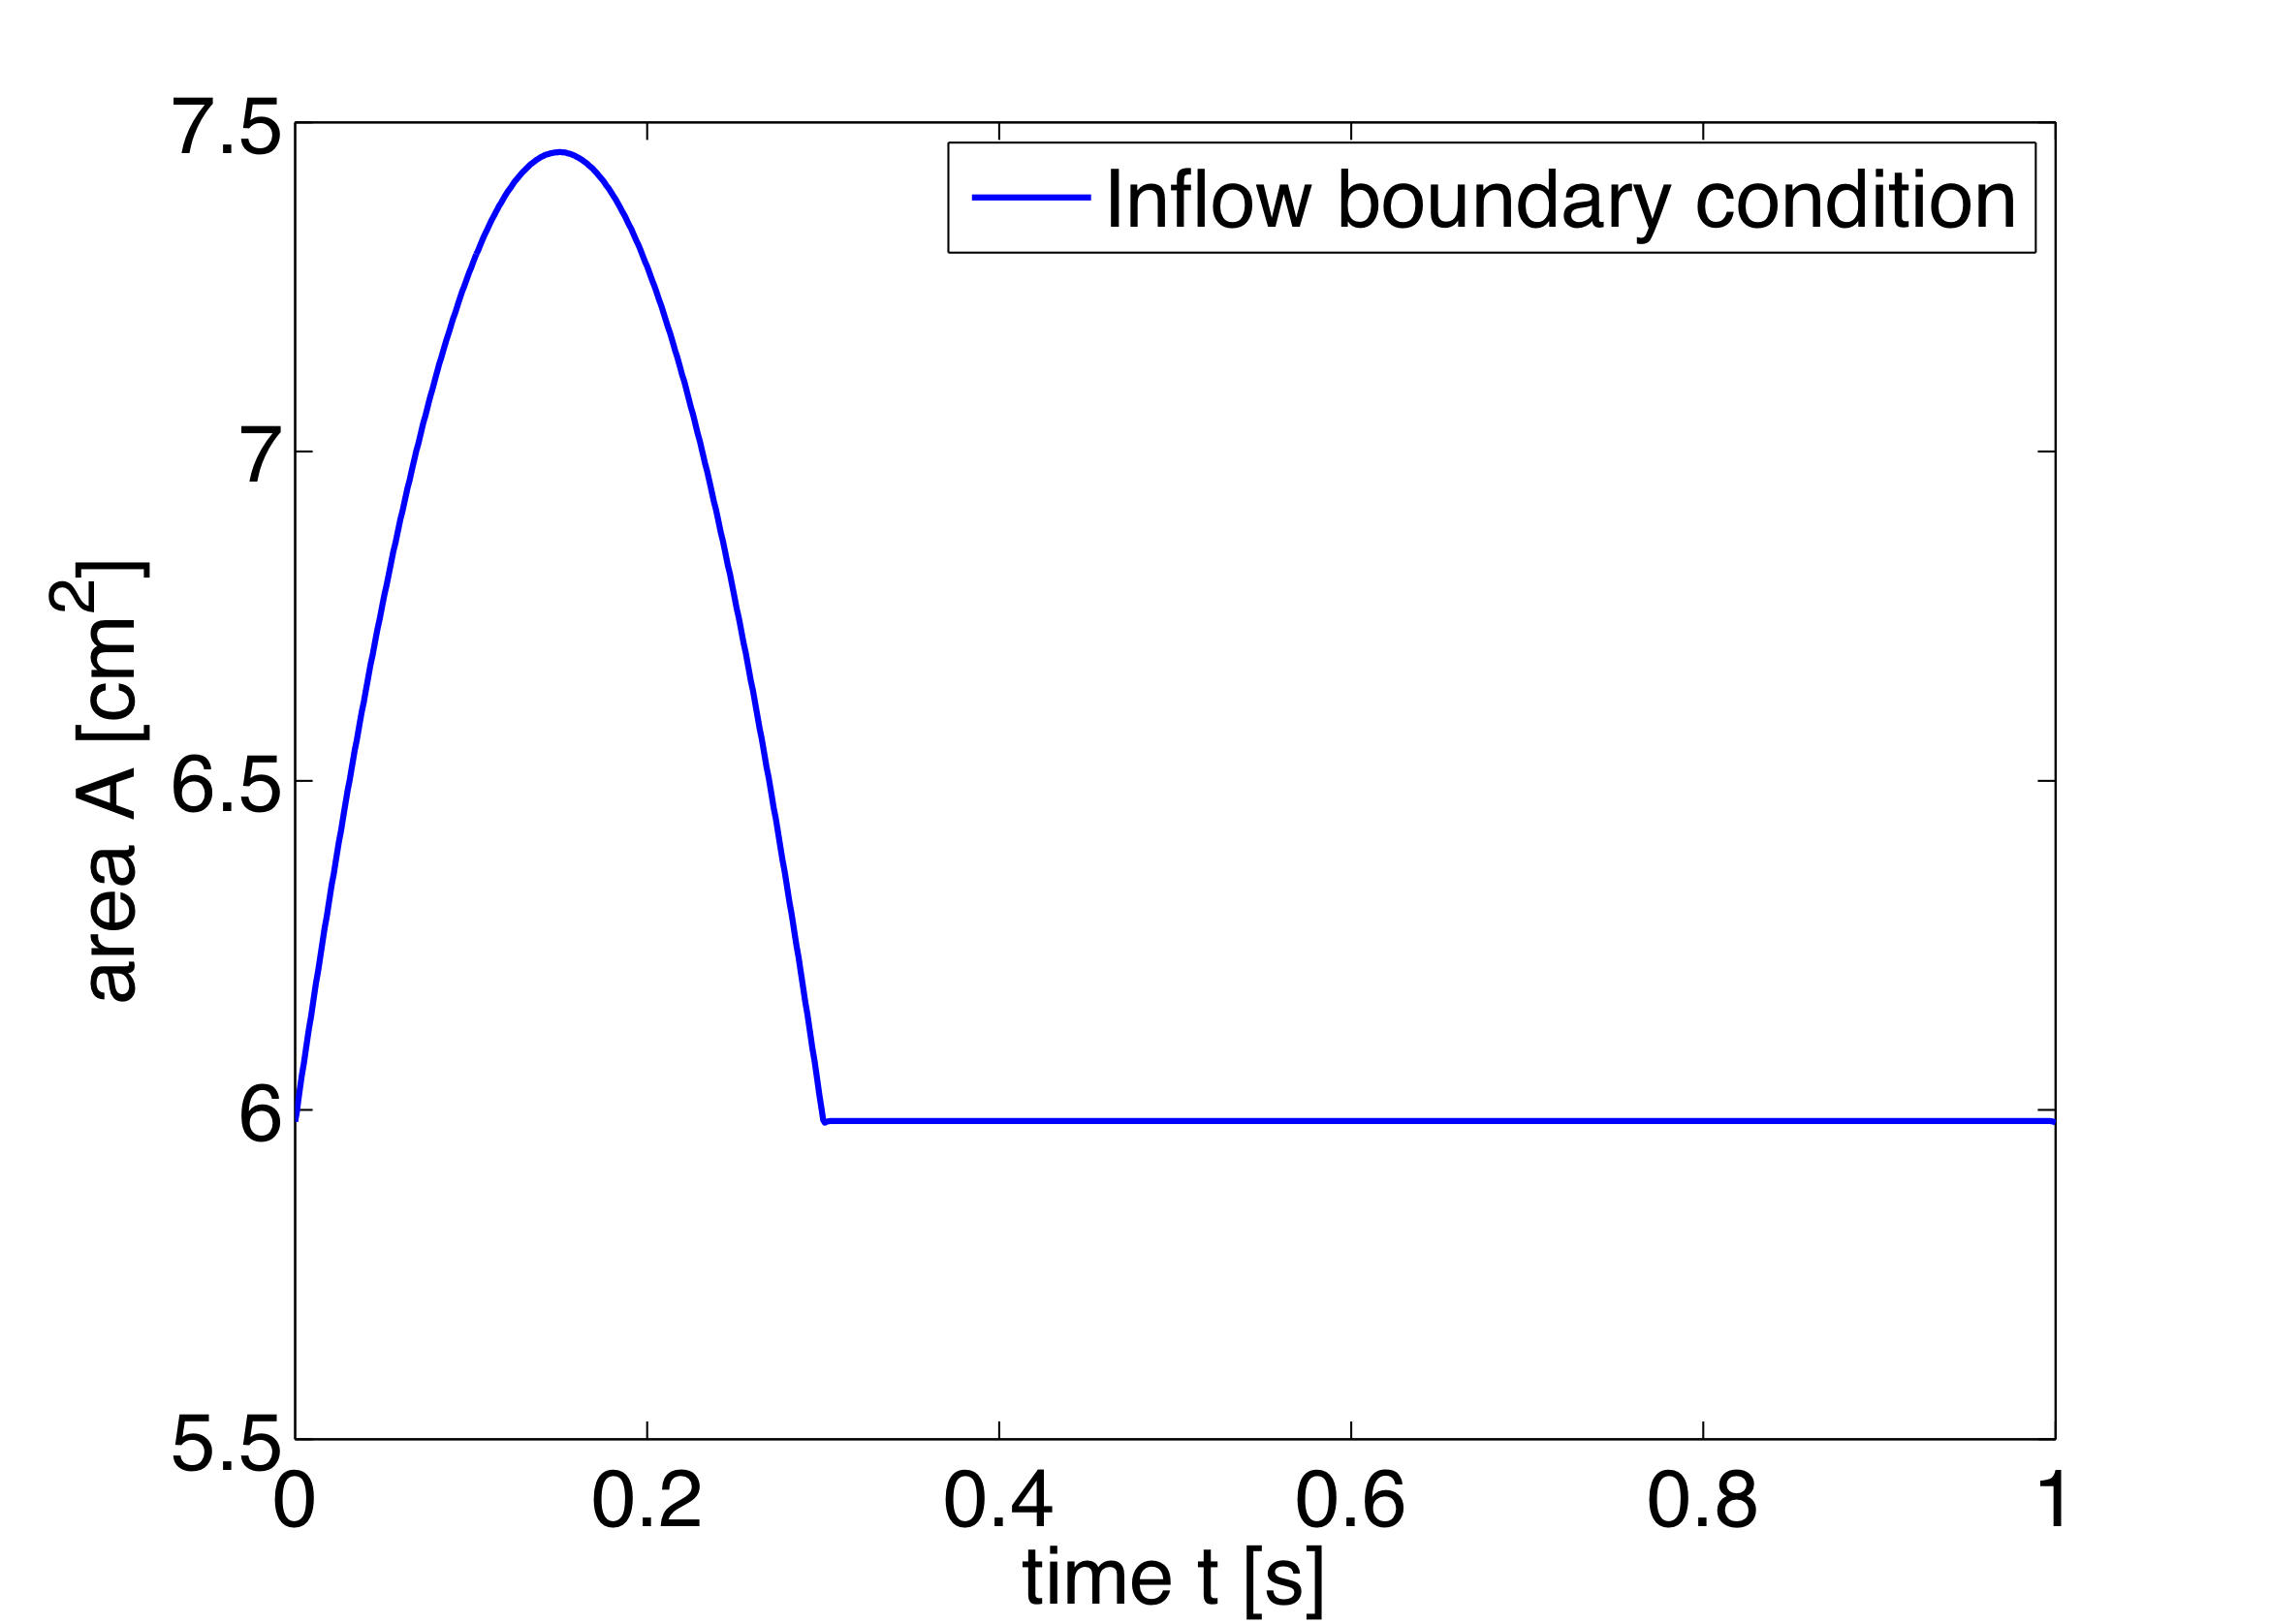
\includegraphics[width=0.49\linewidth]{img/Network_Inflow.png}
\end{figure}

\begin{lstlisting}[style=XmlStyle]
        <BOUNDARYREGIONS>
            <B ID="0"> C[1] </B> <B ID="1"> C[17] </B> <B ID="2"> C[23] </B>
               ...
            <B ID="28"> C[164] </B>
       </BOUNDARYREGIONS>
\end{lstlisting}

In the boundary conditions section the inflow and outflow conditions are set up.
Here we use an inflow boundary condition for the area at the beginning of
the ascending aorta taken from \cite{ShFoPeFr03} and plotted on the
right. Potential choices for inflow boundary conditions include Q-Inflow
and Time-Dependent inflow. The outflow conditions for the terminal regions of
the network could be specified by different models including eTerminal, R, CR,
RCR and Time-Dependant outflow.

\begin{lstlisting}[style=XmlStyle]
<BOUNDARYCONDITIONS>
    <REGION REF="0"> <!-- Inflow -->
        <D VAR="A" USERDEFINEDTYPE="TimeDependent"
           VALUE="5.983*(1+0.597*(sin(6.28*t + 0.628) - 0.588)*
                (1./(1+exp(-2*200*(sin(6.28*t + 0.628) - 0.588)))))" />
        <D VAR="u" USERDEFINEDTYPE="TimeDependent" VALUE="0.0" />
    </REGION>
    <REGION REF="1">
        <D VAR="A" USERDEFINEDTYPE="TimeDependent"  VALUE="A6" />
        <D VAR="u" USERDEFINEDTYPE="TimeDependent"  VALUE="0.0" />
    </REGION>
    <REGION REF="2">
        <D VAR="A" USERDEFINEDTYPE="TimeDependent"  VALUE="A8" />
        <D VAR="u" USERDEFINEDTYPE="TimeDependent"  VALUE="0.0" />
    </REGION>
    <REGION REF="3">
        <D VAR="A" USERDEFINEDTYPE="TimeDependent"  VALUE="A10" />
        <D VAR="u" USERDEFINEDTYPE="TimeDependent"  VALUE="0.0" />
    </REGION>
    ....
    <REGION REF="28">
        <D VAR="A" USERDEFINEDTYPE="TimeDependent"  VALUE="A55" />
        <D VAR="u" USERDEFINEDTYPE="TimeDependent"  VALUE="0.0" />
    </REGION>
</BOUNDARYCONDITIONS>
\end{lstlisting}

Again, for the initial conditions we start our simulation from static
equilibrium conditions $A = A_0$ and for $u$ being initially at rest. The
following lines show how we specify $A_0$ and $\beta$ for different arterial
segments.
\begin{lstlisting}[style=XmlStyle]
<FUNCTION NAME="InitialConditions">
    <E VAR="A" DOMAIN="0" VALUE="5.983" />
    <E VAR="u" DOMAIN="0" VALUE="0.0" />
</FUNCTION>
   ...
<FUNCTION NAME="InitialConditions">
    <E VAR="A" DOMAIN="54" VALUE="A55" />
    <E VAR="u" DOMAIN="54" VALUE="0.0" />
</FUNCTION>

<FUNCTION NAME="A_0">
    <E VAR="A_0" DOMAIN="0" VALUE="A1" />
       ...
    <E VAR="A_0" DOMAIN="54" VALUE="A55" />
</FUNCTION>

<FUNCTION NAME="MaterialProperties">
    <E VAR="beta" DOMAIN="0" VALUE="97" />
      ...
    <E VAR="beta" DOMAIN="54" VALUE="9243" />
</FUNCTION>
\end{lstlisting}

Our simulation is started as described before and the results show the time
history for the conservative variables A and u, as well as for the
characteristic variables W1 and W2 at the beginning of the ascending aorta
(Artery 1). We can see that physically correct the shape of the inflow boundary
condition appears in the forward traveling characteristic W1. As we do not have
a terminal resistance at the outflow, one would normally expect W2 to be
constant. However this is not the case, as bifurcations cause reflections if the
radii of parent and daughter vessels are not well matching, leading to changes
in W2. The shapes of A and u result from this facts and show the values for the
physiological variables during one cardiac cycle. We may annotate that this
values slightly differ from in vivo measurements due to the missing terminal
resistance, which will be added in future.

\begin{figure}
	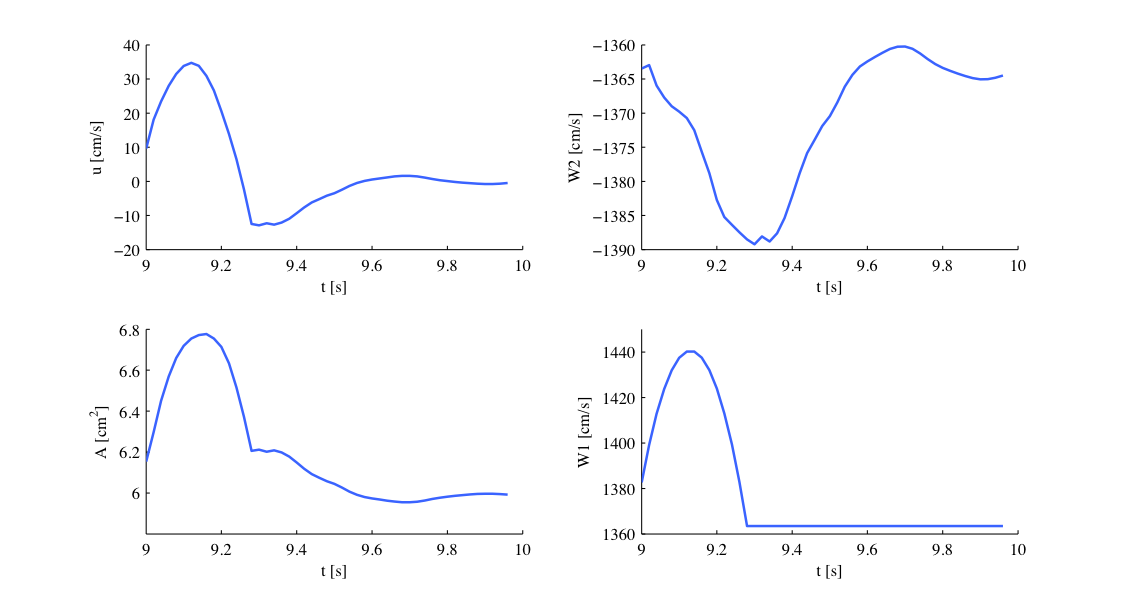
\includegraphics[width=\linewidth]{img/Network_Results.png}
\end{figure}

These short examples should give an insight to the functionality of our
PulseWaveSolver and show that results such as luminal area and pressure within
the artery can be simulated. These results can contribute to understanding the
physiology of the human vascular system and they can be used for
patient-specific planning of medical interventions.

\subsection{Stented Artery}

In the following we will explain the usage of the  \hyperref[PulseWaveSolver]{Pulse Wave solver} to model the flow and pressure variation through a stented artery - a cardiovascular procedure in which a small mesh tube is inserted into an artery to restore blood flow through a constricted region. Due to the implantation of the stent this region will have different material properties compared to the the surrounding unstented tissue; hence will influence the propagation of waves through this system. The stent scenario to be modelled is a straight arterial segment with a stent situated between $x=a_{1}$ and $x=a_{2}$ as shown below.

\begin{figure}
\begin{center}
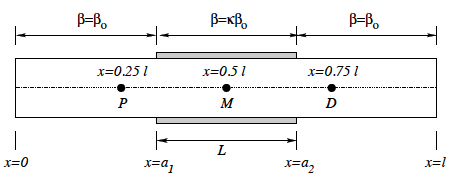
\includegraphics[width=7cm]{img/StentGeometry.png}
\caption{Model of straight artery with a stent in the middle.}
\end{center}
\end{figure}

\paragraph{Geometry:~} In the following we describe the geometry setup for modelling 1D flow in a stent. This is done by defining vertices, elements and composites. The vertices of the domain are shown below, consisting of 30 elements ($\Omega$) and 31 vertices (V[n]).

\begin{figure}
\begin{center}
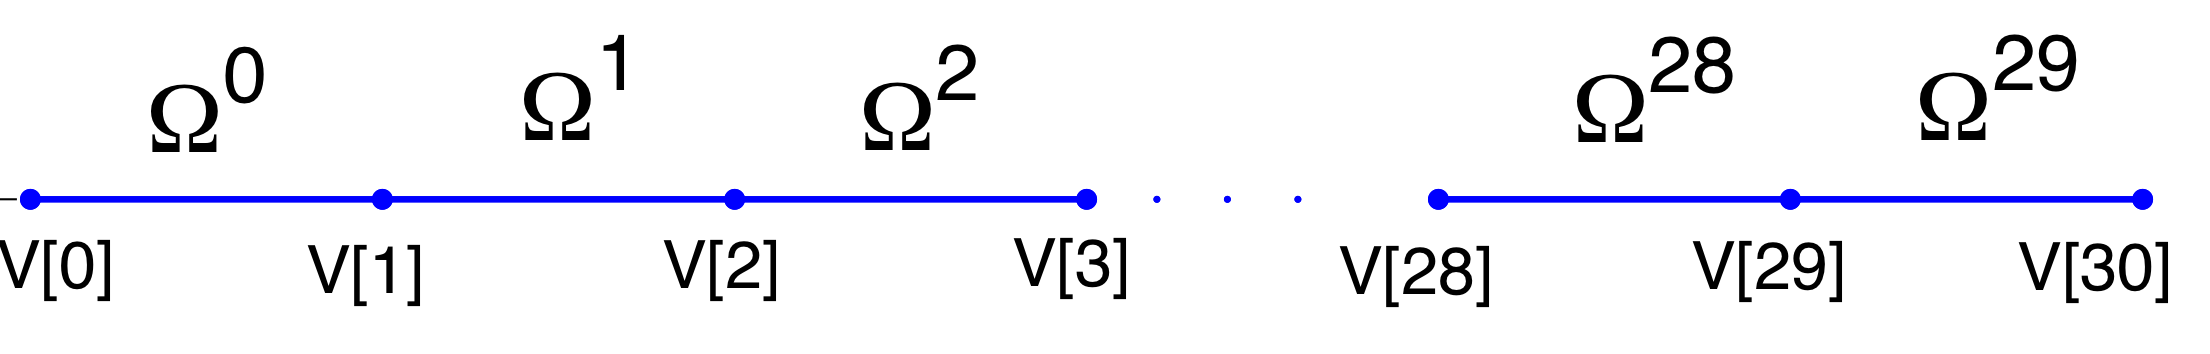
\includegraphics[width=7cm]{img/StentDomain.png}
\caption{1D arterial domain consisting of 30 elements and 31 vertices.}
\end{center}
\end{figure}

To represent the above in the xml file, we define 31 vertices as follows:
\begin{lstlisting}[style=XMLStyle]
<VERTEX>
  <V ID="0"> 0.000e+00 0.000e+00 0.000e+00</V>
               .
               .
               .
  <V ID="30">30.000e+00 0.000e+00 0.000e+00</V>
</VERTEX>
\end{lstlisting}
and the connectivity of these vertices to make up the 30 elements:
\begin{lstlisting}[style=XMLStyle]
<ELEMENT>
  <S ID="0">    0     1 </S>
               .
               .
               .
  <S ID="29">   29    30 </S>
</ELEMENT>
\end{lstlisting}

These elements are combined to three different composites (shown below): composite 0 represents all the elements; composite 1 the inflow boundary and composite 2 the outflow boundary.

\begin{figure}
\begin{center}
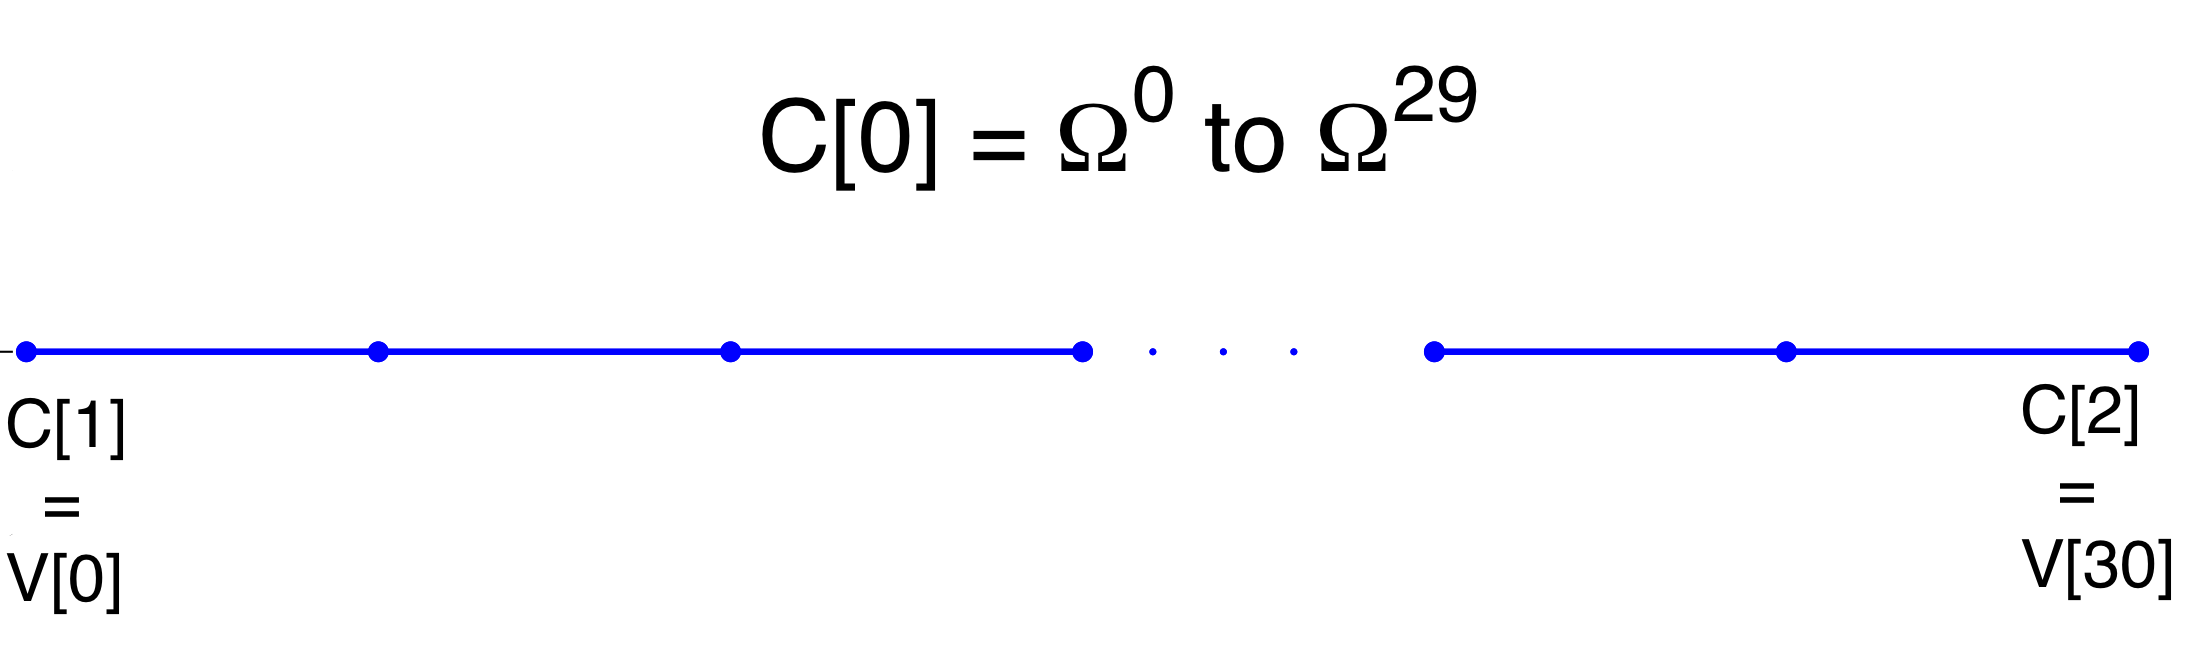
\includegraphics[width=7cm]{img/StentComposite.png}
\caption{Three composites (C[0], C[1] and C[2]) for the stunted artery.}
\end{center}
\end{figure}

The above composites are specified as follows:
\begin{lstlisting}[style=XMLStyle]
<COMPOSITE>
  <C ID="0"> S[0-29] </C>
  <C ID="1"> V[0] </C>
  <C ID="2"> V[30] </C>
</COMPOSITE>
\end{lstlisting}

Finally the domain is specified by the first composite by
\begin{lstlisting}[style=XMLStyle]
<DOMAIN>
  <D ID="0"> C[0] </D>
</DOMAIN>
\end{lstlisting}

\paragraph{Expansion:~}For the expansions we use 4th-order polynomials which define our two variables A and u on the domain.

\begin{lstlisting}[style=XMLStyle]
<EXPANSIONS>
  <E COMPOSITE="C[0]" NUMMODES="5" FIELDS="A,u" TYPE="MODIFIED" />
</EXPANSIONS>
\end{lstlisting}

\paragraph{Time Integration Scheme:~} For the Time Integration Scheme
we use a basic Forward Euler method.

\begin{lstlisting}[style=XMLStyle] 
<TIMEINTEGRATIONSCHEME>
  <METHOD> ForwardEuler </METHOD>
  <ORDER> 1 </ORDER>
</TIMEINTEGRATIONSCHEME>
\end{lstlisting}
        
\paragraph{Solver Information:~}The Discontinuous Galerkin Method is used as projection scheme and the time-integration is performed by a simple Forward Euler scheme. A full list of possible time integration scheme is given in the parameter section of the  \hyperref[PulseWaveSolver]{Pulse Wave Solver}
\begin{lstlisting}[style=XMLStyle]
<SOLVERINFO>
  <I PROPERTY="EQTYPE" VALUE="PulseWavePropagation" />
  <I PROPERTY="Projection" VALUE="DisContinuous" />
  <I PROPERTY="TimeIntegrationMethod" VALUE="ForwardEuler" />
  <I PROPERTY="UpwindTypePulse"  VALUE="UpwindPulse"/>
</SOLVERINFO>
\end{lstlisting}

\paragraph{Parameters:~} Parameters used for the simulation are taken from \cite{ShFoPeFr03}
\begin{lstlisting}[style=XMLStyle]
<PARAMETERS>
   <P> TimeStep       = 2e-6               </P>
   <P> FinTime        = 0.25               </P>
   <P> NumSteps       = FinTime/TimeStep   </P>
   <P> IO_CheckSteps  = NumSteps/50        </P>
   <P> IO_InfoSteps   = 100                </P>
   <P> T              = 0.33               </P>
   <P> h0             = 1.0                </P>
   <P> rho            = 1.0                </P>
   <P> nue            = 0.5                </P>
   <P> pext           = 0.0                </P>
   <P> a1             = 10.0               </P>
   <P> a2             = 20.0               </P>
   <P> kappa          = 100.0              </P>
   <P> Y0             = 1.9099e+5          </P>
   <P> k              = 2                  </P>
   <P> k1             = 200                </P>
 </PARAMETERS>
\end{lstlisting}

\paragraph{Boundary conditions:~} At the inflow we apply a pressure boundary condition as shown in the figure below. This condition models the pressure variation during one heartbeat. A simple absorbing outflow boundary condition is applied the right end of the tube.

\begin{figure}
\begin{center}
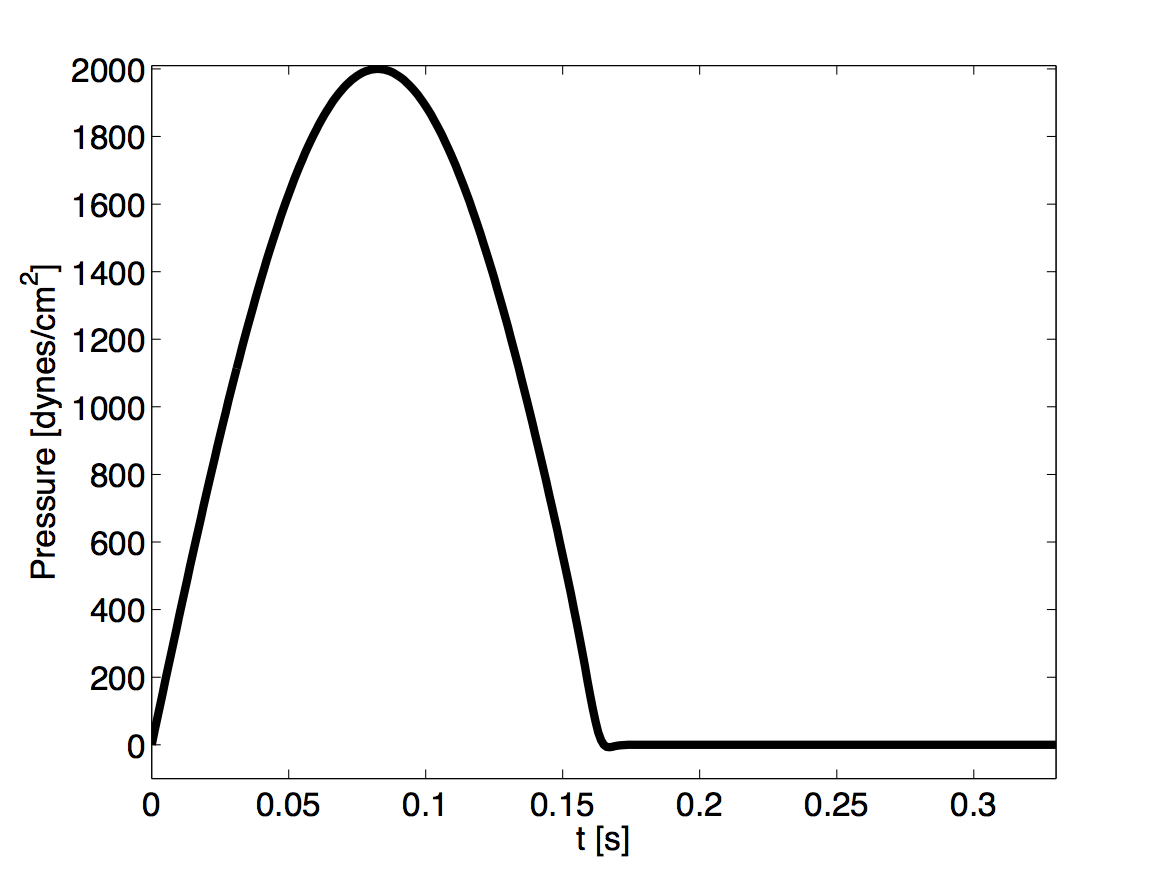
\includegraphics[width=7cm]{img/StentPressureProfile.png}
\caption{Pressure profile applied at the inlet of the artery}
\end{center}
\end{figure}

These are defined in the xml file as follows,
\begin{lstlisting}[style=XMLStyle]
<BOUNDARYREGIONS>
   <B ID="0"> C[1] </B>
   <B ID="1"> C[2] </B>
</BOUNDARYREGIONS>

<BOUNDARYCONDITIONS>
   <REGION REF="0">
      <D VAR="A" USERDEFINEDTYPE="TimeDependent" VALUE=
      "(2000*sin(2*PI*t/T)*1./(1+exp(-2*k1*(T/2-t))-pext)/451352+1)^2" />
      <D VAR="u" USERDEFINEDTYPE="TimeDependent" VALUE="1.0" />
   </REGION>
   <REGION REF="1">
      <D VAR="A" VALUE="1.0" />
      <D VAR="u" VALUE="1.0" />
   </REGION>
</BOUNDARYCONDITIONS>
\end{lstlisting}

The simulation starts from the static equilibrium of the vessel with normalised area and velocity.
\begin{lstlisting}[style=XMLStyle]
<FUNCTION NAME="InitialConditions">
	<E VAR="A" DOMAIN="0" VALUE="1.0" />
	<E VAR="u" DOMAIN="0" VALUE="1.0" />
</FUNCTION>

<FUNCTION NAME="A_0">
	<E VAR="A" DOMAIN="0" VALUE="1.0" />
</FUNCTION>
\end{lstlisting}

\paragraph{Functions:~} The stent is introduced by applying a variable material properties function ($\beta$ - see Eq. \eqref{eqn:PA}) along the vessel in the x direction, shown graphically below
\begin{figure}
\begin{center}
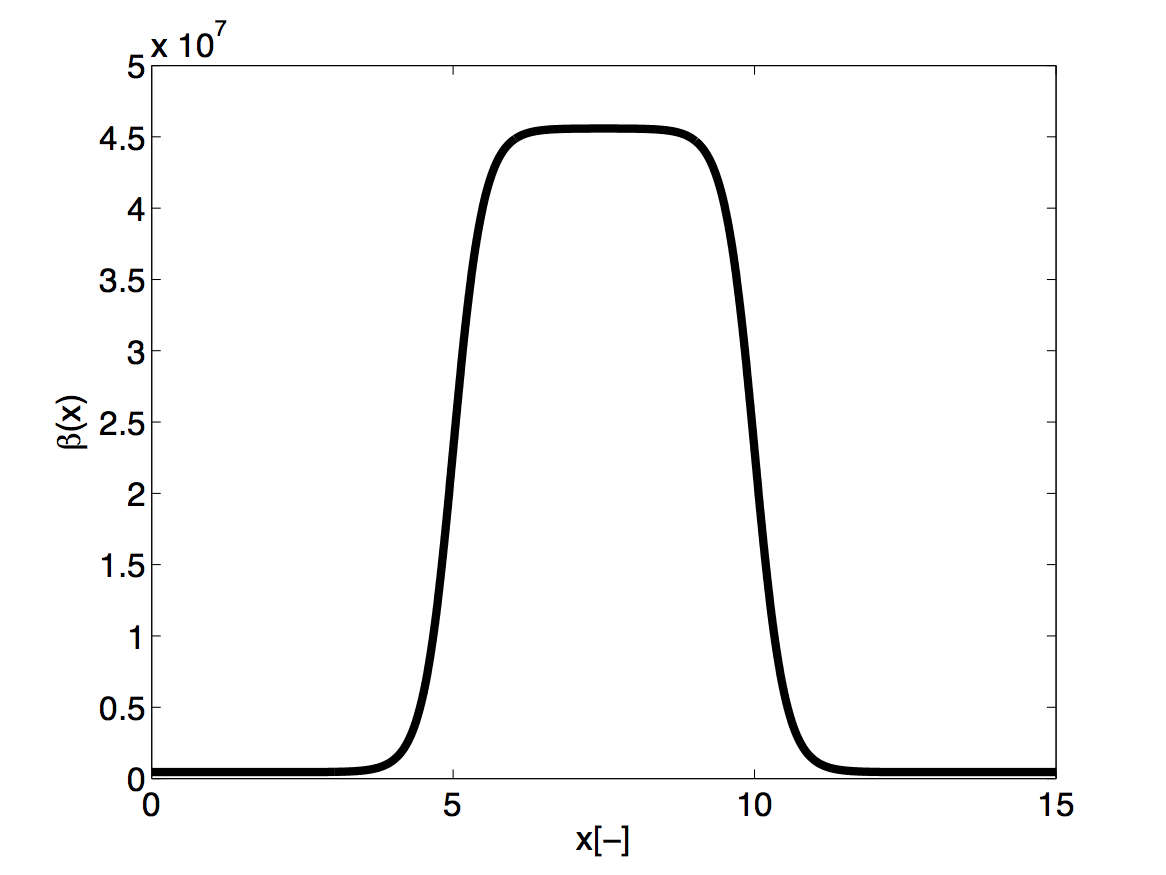
\includegraphics[width=7cm]{img/StentMaterial.png}
\caption{material property variation along the artery. The stiff region in the middle represents the stent.}
\end{center}
\end{figure}
and defined in the xml file by
\begin{lstlisting}[style=XMLStyle]
<FUNCTION NAME="MaterialProperties">
	<E VAR="E0" DOMAIN="0" VALUE=
	"Y0*(1.0-kappa/(1+exp(-2*k*(a1-x)))+kappa/(1+exp(-2*k*(a2-x))))" />
</FUNCTION>
\end{lstlisting}

\subsubsection{Simulation}
The simulation is started by running
\begin{lstlisting}[style=BashInputStyle]
PulseWaveSolver Test_1.xml
\end{lstlisting}
It will take about 60 seconds on a 2.4GHz Intel Core 2 Duo processor and
therefore is computationally realisable at every clinical site.

\subsubsection{Results}
As a result we get a 3-dimensional interpretation of the aortic cross-sectional
area varying in axial direction both for the stented and non-stented vessel. In
case of the stent, the rigid metal mesh will restrict the deformation of the
area in that specific part of the artery compared to the normal vessel
(Fig.~\ref{f:pulsewave:stented:vessels}).

\begin{figure}
	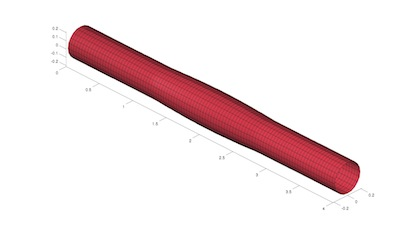
\includegraphics[width=0.49\linewidth]{img/normal_vessel.jpg}
	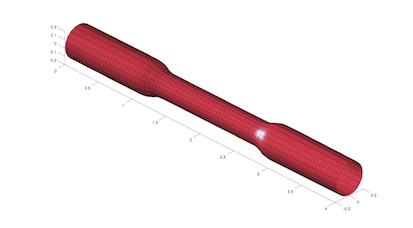
\includegraphics[width=0.49\linewidth]{img/stented_vessel.jpg}
	\caption{}
	\label{f:pulsewave:stented:vessels}
\end{figure}

Also, if we look at the pressure at three points within the artery (P, M, D) we
will recognize that there are major differences between the stented and normal
vessel. While in the normal vessel (left) the pressure wave applied at the
inflow is propagated without any losses, this does not hold for the stented
artery (right). Here, the stiffening at the stent causes reflections and thus
there are losses for total pressure at the medial (M) and distal (D) point.

\begin{figure}
	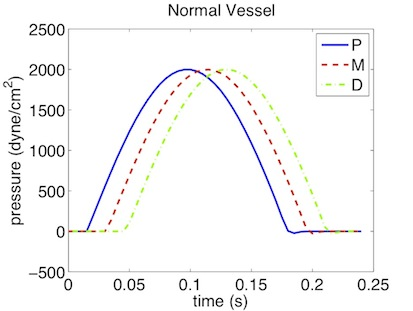
\includegraphics[width=0.49\linewidth]{img/pressure_normal_vessel.jpg}
	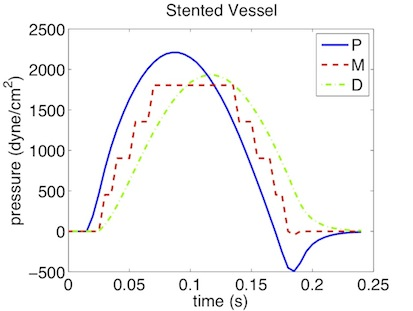
\includegraphics[width=0.49\linewidth]{img/pressure_stented_vessel.jpg}
\end{figure}

\section{Further Information}
The PulseWaveSolver has been developed with contributions by various students
and researchers at the Department of Aeronautics, Imperial College London.
Further information on the solver and its underlying mathematical framework
can be found in \cite{Ro12,Pi12}.

\section{Future Development}
The PulseWaveSolver is a useful tool for computational modelling of
one-dimensional blood flow in the human body. However, there are several ideas
for future development which include:
\begin{enumerate}
\item Inclusion of a pre-processor and post-processor.
\item Profiling the code to improve performance.
\item Cleaning up the input file to make the input format more user-friendly.
\item Modelling of valves and alternative pressure-area laws for models of
venous flow.
\item Incorporating a model of the heart.
\end{enumerate}

\section{References}

\noindent [1] Reavette R, Sherwin SJ, Tang MX, Weinberg PW. Comparison of arterial wave intensity analysis by pressure-velocity and diameter-velocity methods in a virtual population of adult aubjects.\textit{ Journal of Engineering in Medicine}. 2020.

\noindent [2] Alastruey J. Numerical modelling of pulse wave propagation in the cardiovascular system: development, validation and clinical applications. \textit{PhD thesis, Imperial College London}. 2006.

% These are unreferenced citations
% N. Westerhof et al., Anatomic studies of the human systemic arterial tree, J.
% Biomech. 2:121-143, 1969 Three-dimensional blood flow profile in a rabbit aorta done with Nektar++,
% courtesy of Véronique Peiffer
